\documentclass{article}
% Babel is used fot language
\usepackage[english]{babel}
\usepackage{tikz}
% Geometry is used for margin and general lenghts
\usepackage[xetex,
            a4paper,
            top    = 0.50cm,
            left   = 0.5in,
            right  = 0.7in,
            bottom = 0.50cm]{geometry}

%font packages
\usepackage[utf8]{inputenc}
\usepackage[T1]{fontenc}
\usepackage{fontspec}
\usepackage{fontawesome5}
\usepackage[default]{raleway}

%progressbar
\usepackage[roundnessr   = 0.40,
            width        = 10em,
            subdivisions = 1,
            emptycolor   = C1,
            filledcolor  = C2 ]{progressbar}

% Images using graphicx and subfigures using subcaption
\usepackage{graphicx}
\graphicspath{ {imgs/} }
\usepackage[font=small,labelfont=bf]{subcaption}

% Pretty Table formatting
\usepackage{booktabs}

% Multicolumns
\usepackage{multicol}

%URL
\usepackage[pdfauthor = {Giuseppe Minardi},
            colorlinks,
            linkcolor = black,
            citecolor = black,
            urlcolor  = black]{hyperref}

% Icons
% Color
\usepackage{xcolor}
\definecolor{C1}{RGB}{58,51,53}
\definecolor{C2}{RGB}{229,88,18}
\definecolor{C3}{RGB}{225,81,84}

% Multcolumn
\usepackage{multicol}

% Evental title formatting
\usepackage{titlesec}
\titleformat{\section}{\Large\bfseries\scshape\color{C1}}{}{1em}{}[\color{C2}{\titlerule[2.5pt]}]
\titleformat{\subsection}{\large\bfseries\color{C3}}{}{0.2\textwidth}{}
\titleformat{\subsubsection}{\bfseries\itshape}{}{0pt}{}

\newcommand{\entry}[4]{
    \begin{minipage}[b]{.25\textwidth}
        \begin{raggedleft}

            \textbf{#1}

        \end{raggedleft}



    \end{minipage}
    \hfill\vline\hfill
    \begin{minipage}[c]{.7\textwidth}


        \textbf{#2}

        \textit{#3}

        #4


    \end{minipage}
    \\[1ex]
}

\newcommand{\slimentry}[3]{
    \begin{minipage}[c]{.35\textwidth}
        \begin{raggedleft}

            \textit{#1}

        \end{raggedleft}



    \end{minipage}
    \hfill\vline\hfill
    \begin{minipage}[c]{.6\textwidth}


        \textbf{#2}. #3




    \end{minipage}
    \\[1ex]
}


\newcommand{\thesisentry}[3]{
    \begin{minipage}[b]{.25\textwidth}
        \begin{raggedleft}

            \textbf{#1}

        \end{raggedleft}



    \end{minipage}
    \hfill\vline\hfill
    \begin{minipage}[c]{.7\textwidth}


        \begin{description}

            \item[Title] ``#2''
            \item[Description] \textit{#3}

        \end{description}


    \end{minipage}
    \\[1ex]
}

%========================================================================
\renewcommand{\maketitle}{

	\begin{minipage}[c]{.5\textwidth}
        \begin{center}
            \Huge \textbf{Giuseppe Minardi}


        \end{center}


	\end{minipage}
    \hfill\hfill
    \begin{minipage}[c][3.5cm]{.5\textwidth}

        \vfill

        \faHome\hspace{0.3cm} Trento (TN), 38122, Italy

        \faPhone\hspace{0.3cm}+39 389 178 5933

        \href{mailto:giuseppe.minardi95@gmail.com}{\faEnvelope\hspace{0.3cm}giuseppe.minardi95@gmail.com}

        \faSkype\hspace{0.3cm} minardi.giuseppe

        \faLinkedin\hspace{0.3cm} \url{linkedin.com/in/giuseppeminardi95}

	\end{minipage}
}
%========================================================================
\newcommand{\uot}{University of Trento}

\begin{document}
\pagenumbering{gobble}
\urlstyle{same}
\maketitle

	\begin{minipage}[t]{.6\textwidth}

\section{Experiences}

\subsection{Job Experiences}


        \entry{02/2018--06/2019}{Organic Chemistry Tutor}{\uot, Trento (TN)}{}

        \entry{06/2017--07/2017}{Internship}{Novartis s.p.a.}{My Bachelor Thesis is based on this experience}

        \entry{11/2016--03/2017}{Collaboration}{\uot, Trento (TN)}{Search and classification of \textit{research grants} to be used by CIBio's researchers.}


\subsection{Volunteering Experiences}

\entry{2015--2016}{Member of Staff}{OWL -- Open Wet Lab}{First biohacking group in Italy}
\entry{2018--2019}{Volunteer}{UNITiN}{UNITiN is an SGA that operates in all departments of the \uot.}

\section{Education}


        \entry{2017--2019} {\textsc{M.S.C.B.} ~ Quantitative and Computational Biology}{\uot, Trento (TN)}{\textbf{Thesis:}~ An innovative bioinformatic approach to select new targets for antimicrobial therapies.}

        \entry{2014--2017}{\textsc{B.S.Biotech} ~ Biomolecular Sciences and Technologies}{\uot, Trento (TN)}{\textbf{Thesis:} Assessment of the optimal levels of calcium and phosphate ions in the tgrowth of Streptomyces \textit{clavuligerus} and its production of Clavulanic Acid.}


    \end{minipage}
    \hfill
    {\color{C1}\vrule}
    \hfill
	\begin{minipage}[t]{.35\textwidth}


\section{Languages}

    \slimentry{Italian}{\progressbar{1.0}}{}
\slimentry{English}{\progressbar{0.8}}{}

\section{Technical skills}

        \slimentry{Linux}{\progressbar{0.85}}{}
        \slimentry{Windows and MacOS}{\progressbar{0.9}}{}
        \slimentry{MS Office}{\progressbar{0.9}}{}
        \slimentry{Markdown and \LaTeX}{\progressbar{0.9}}{}
        \slimentry{R and Python}{\progressbar{0.7}}{}
        \slimentry{Data analysis}{\progressbar{0.80}}{}
        \slimentry{Machine Learning}{\progressbar{0.70}}{}
        \slimentry{Clustering}{\progressbar{0.7}}{}
        \slimentry{Classification}{\progressbar{0.8}}{}
        \slimentry{Regression}{\progressbar{0.70}}{}
        \slimentry{Statistics}{\progressbar{0.80}}{}
        \slimentry{Bioinformatics}{\progressbar{0.90}}{}
        \slimentry{Genomics}{\progressbar{0.80}}{}


\section{Soft Skills}
\resizebox{\columnwidth}{!}{%
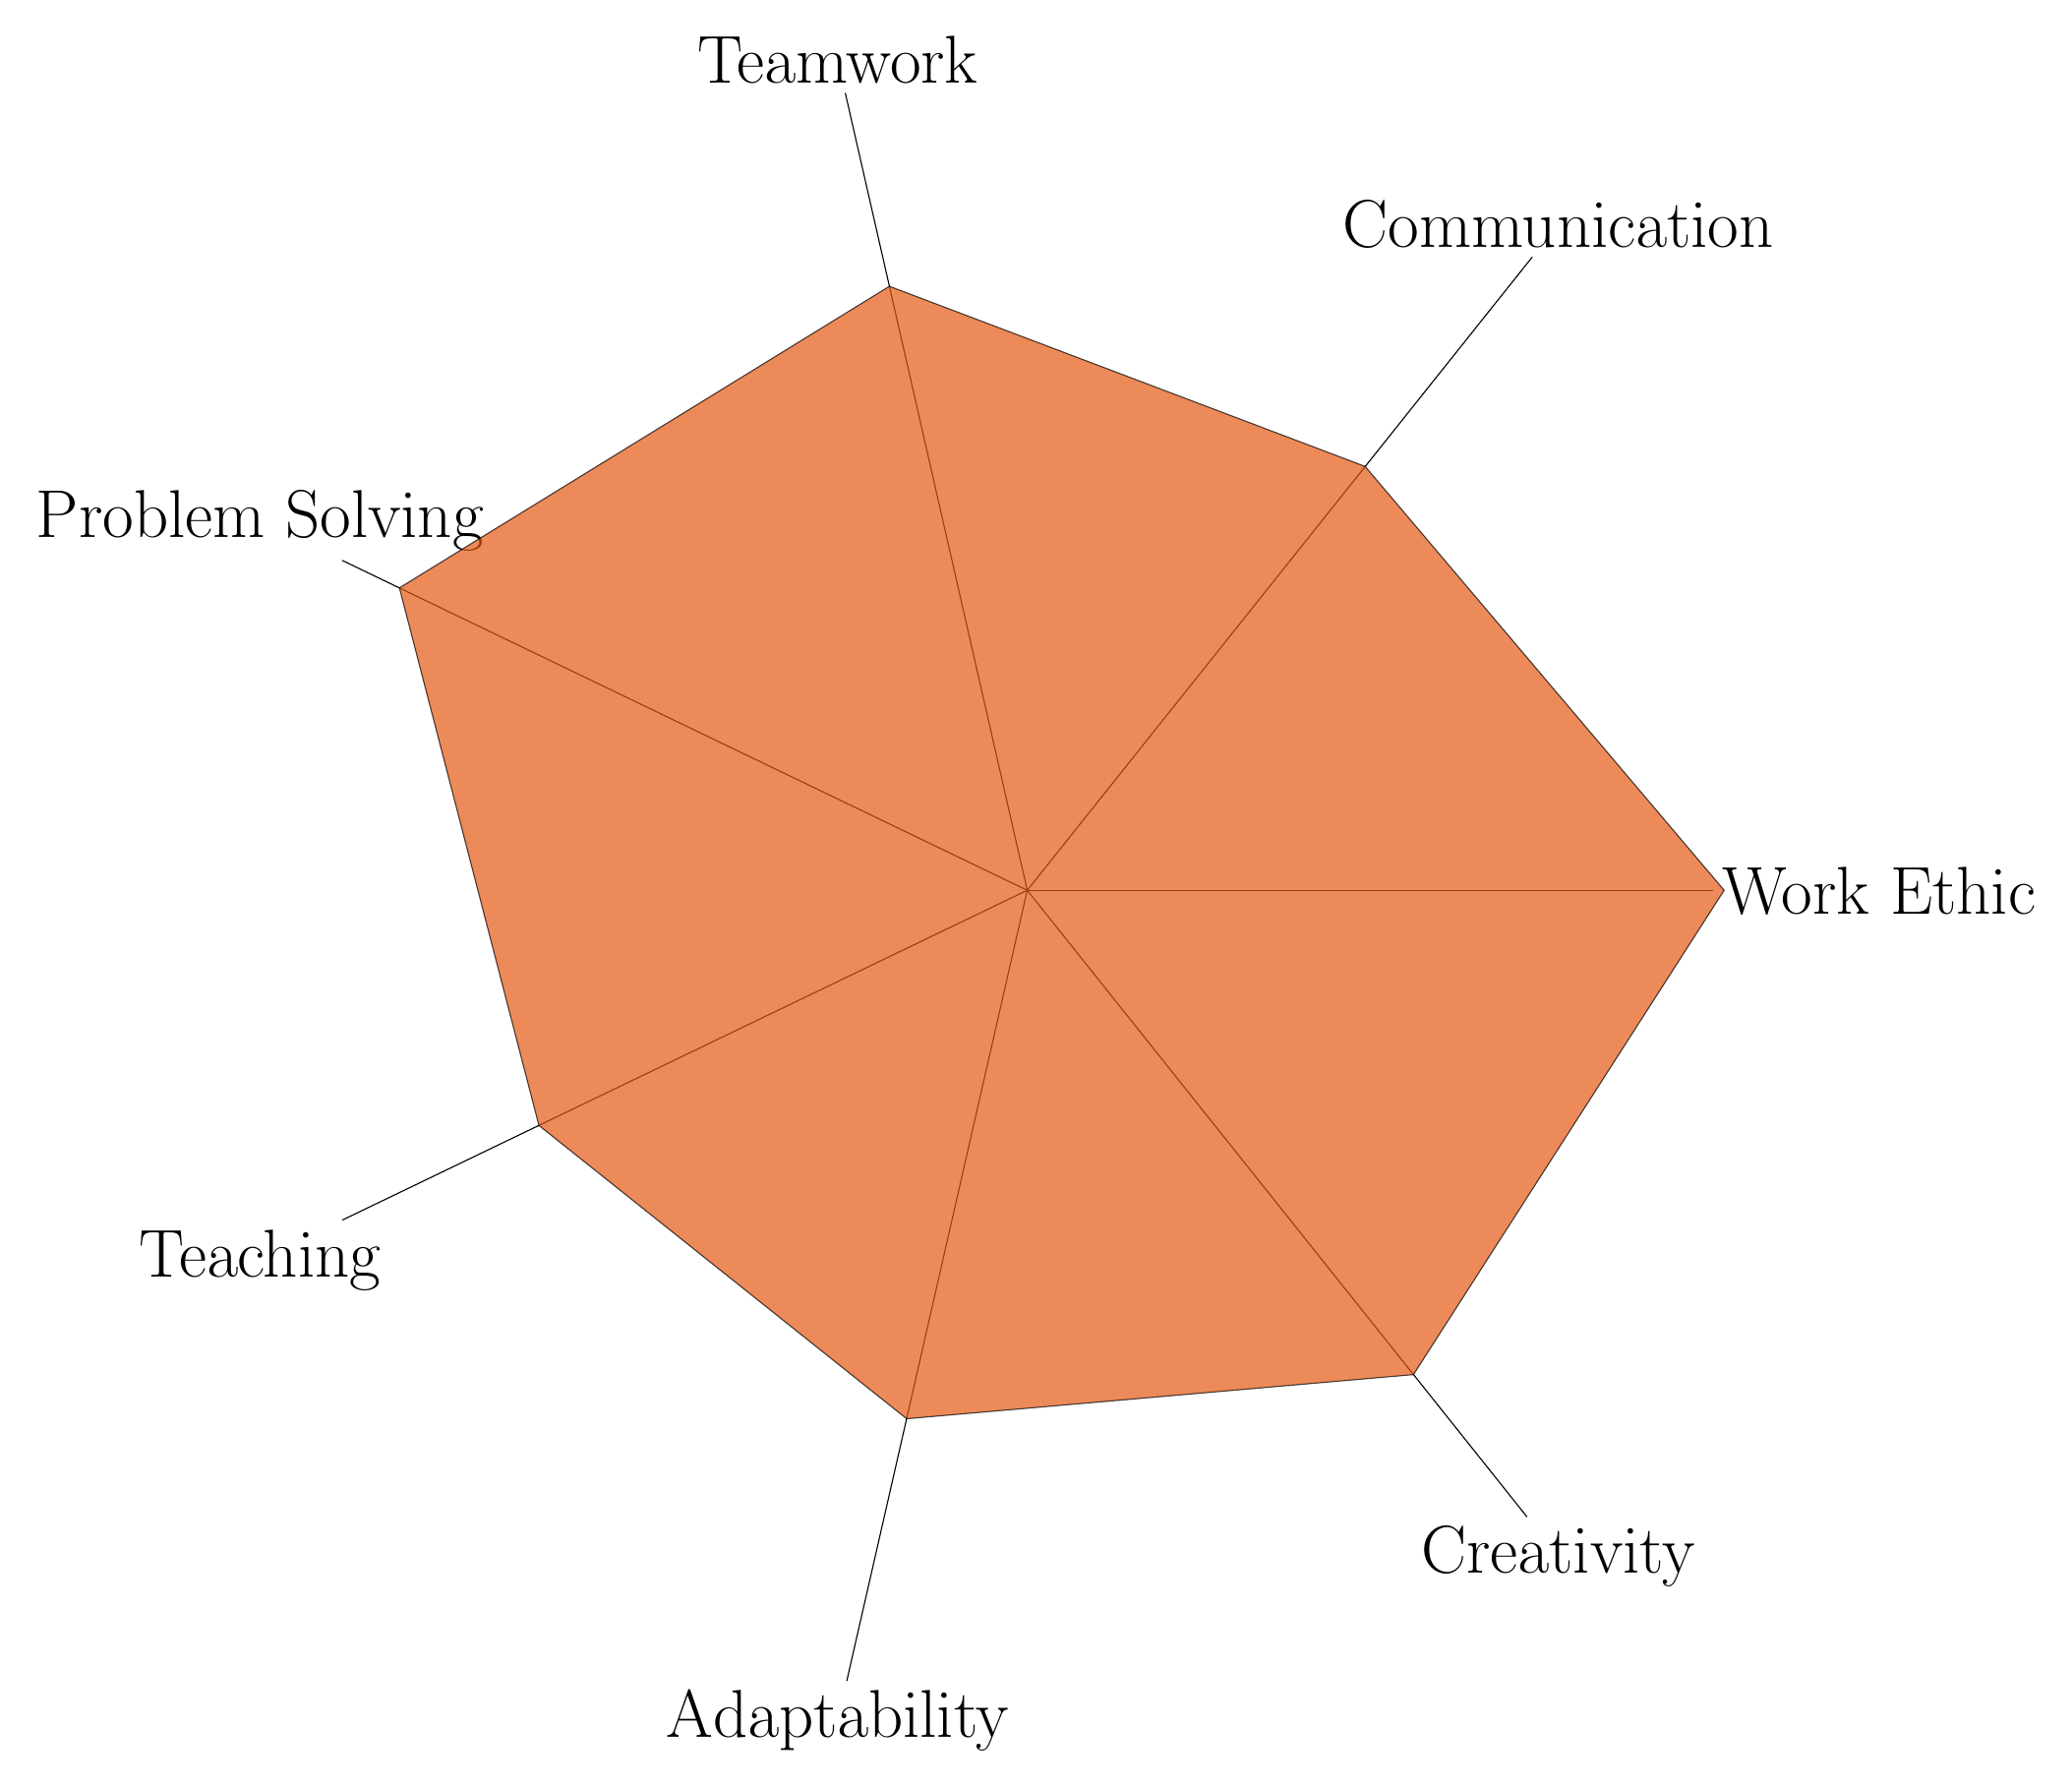
\begin{tikzpicture}
    \coordinate (origin) at (0, 0);

    \foreach[count=\i] \radius/\dim in {7/Communication,
                                        8/Teamwork,
                                        9/Problem Solving,
                                        7/Teaching,
                                        7/Adaptability,
                                        8/Creativity,
                                        9/Work Ethic}{
        \coordinate (\i) at (\i * 360 / 7: \radius);
        \node (title) at (\i * 360 / 7: 11) {\Huge\dim};
        \draw (origin) -- (title);
    }

    \draw [fill=C2, opacity=.7] (1)
                                \foreach \i in {2,...,7}{-- (\i)} --cycle;
\end{tikzpicture}}



\section{Other Interests}
Music, Astronomy, Economics, Technology

    \end{minipage}
\end{document}
